\section{Equations of Motion Derivation}

To derive the equations of motion, solve a force-balance for the kinetic equations, then use geometry to develop the kinematic equations and substitute these into the kinetic equations.

\subsection*{Kinetic Equations}

The kinetic equations are formulated by equating the free-body diagram (FBD) with the mass-acceleration diagram as shown in Figure~\ref{FBD=MAD}. The stiffening unit $x$- and $y$-force vector directions are determined by assuming the mirror is displaced in the positive respective direction with positive respective velocity, then inferring the restoring and resistive force imparted by each stiffening unit. The disturbance forces are defined as positive in the $+x$- and $+y$-directions. Referring to the stiffener diagram of Figure~\ref{stiff}, a force-balance for each identical unit as shown in Equation~\eqref{eq:stiffener} characterizes the reactive force at each node.

\begin{equation}
\label{eq:stiffener}
\begin{aligned}
		\sum{F} &= m\ddot{s}\\
		0 &= S - ks - c\dot{s}\\
		S &= ks + c\dot{s}
\end{aligned}
\end{equation}\

\begin{figure}	% FBD=MAD
 \centering
 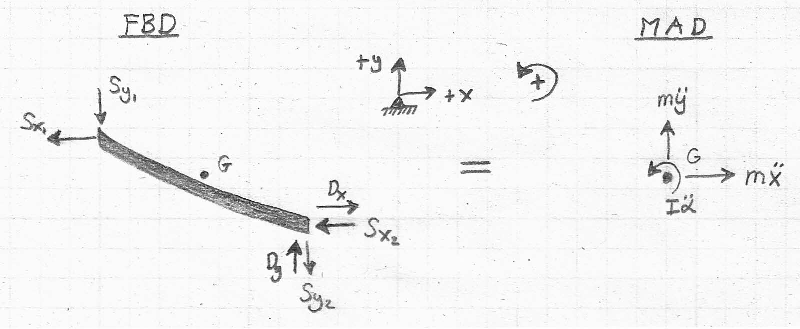
\includegraphics[width=0.75\textwidth]{Figures/Q5_P1_FBD=MAD.pdf}
 \caption{Set the free-body diagram equal to the mass-acceleration diagram to formulate the kinetic equations}
 \label{FBD=MAD}
\end{figure}

\begin{subequations}
\label{eq:kinEQ}
\begin{align}
	\begin{split}
	\sum{F_x} &= m\ddot{x} \\
	m\ddot{x} &= -S_{x_1}-S_{x_2}+Dx \\
	m\ddot{x} &= -kx_1 - c\dot{x_1} - kx_2 - c\dot{x_2} + D_x \\
	\end{split}\\
	\begin{split}
	\sum{F_y} &= m\ddot{y}\\
	m\ddot{y} &= -S_{y_1}-S_{y_2}+Dx \\
	m\ddot{y} &= -ky_1 - c\dot{y_1} - ky_2 - c\dot{y_2} + D_y\\
	\end{split}\\
	\begin{split}
	\sum{M_G} &= I\ddot{\alpha}\\
	I\ddot{\alpha} &= \rho_{2_y}\left[-S_{x_2}+D_x\right] +  \rho_{2_x}\left[-S_{y_2}+D_y\right] + \rho_{y_1}S_{x_1} + \rho_{x_1}S_{y_1}  \\
	I\ddot{\alpha} &= \rho_{2_y}\left[-kx_2 - c\dot{x}_2+D_x\right] +  \rho_{2_x}\left[-ky_2 - c\dot{y}_2+D_y\right] + \rho_{1_y}\left[-kx_1 - c\dot{x}_1\right] + \rho_{1_x}\left[-ky_1 - c\dot{y}_1\right]  \\
	\end{split} \\ \nonumber
\end{align}
\end{subequations}

\subsection*{Kinematic Equations}

The kinematic equations define the interdependencies of the motion of the state variables. For this simulation, these are defined by the geometry of the mechanical system. Specifically, these equations define the positions and velocities of the mirror segment endpoints by the mirror segment CoM position, velocity, and rotation angle.

\begin{equation}
\label{eq:kinemEQ}
\begin{aligned}
		x_1 &= x - d\rho_{1_x} & x_2 &= x + d\rho_{2_x} \\
		\dot{x_1} &= \dot{x} - d\dot{\rho}_{1_x} & \dot{x_2} &= \dot{x} + d\dot{\rho}_{2_x} \\
		y_1 &= y - d\rho_{1_y} & y_2 &= y + d\rho_{2_y} \\
		\dot{y_1} &= \dot{y} - d\dot{\rho}_{1_y} & \dot{y_2} &= \dot{y} + d\dot{\rho}_{2_y}
\end{aligned}
\end{equation}

Where

\begin{equation}
\centering
	\begin{aligned}
	d\rho_{1_x} &= d\rho_1\cos\left( \phi_1 \right) & d\rho_{2_x} &= d\rho_2\cos\left( \phi_2 \right)\\
	d\dot{\rho}_{1_x} &= d\dot{\rho}_1\cos\left( \phi_1 \right) & d\dot{\rho}_{2_x} &= d\dot{\rho}_2\cos\left(\phi_2\right)\\
	d\rho_{1_y} &= d\rho_1\sin\left( \phi_1 \right) & d\rho_{2_y} &= d\rho_2\sin\left( \phi_2 \right)\\
	d\dot{\rho}_{1_y} &= d\dot{\rho}_1\sin\left( \phi_1 \right) & d\dot{\rho}_{2_y} &= d\dot{\rho}_2\sin\left(\phi_2\right)	
	\label{eq:drho}
	\end{aligned}
\end{equation}\

 For this simulation, all rotations about the CoM, $\alpha$, are small enough that the small-angle approximation, Equation~\eqref{eq:smallAngle}, is assumed valid.

\begin{equation}
\centering
	\begin{aligned}
	d\vec{\rho} &\approx \vec{\rho}\sin \left(\alpha\right) &\approx \vec{\rho}\alpha \\
	d\dot{\vec{\rho}} &\approx \vec{\rho} \left[d\left(\sin \left(\alpha\right)\right)\right] &\approx  \vec{\rho}\dot{\alpha}
	\label{eq:smallAngle}
	\end{aligned}
\end{equation}

Such that,

\begin{equation}
\centering
	\begin{aligned}
	d\rho_{1_x} &= \rho_1\alpha\cos\left( \phi_1 \right) & d\rho_{2_x} &= \rho_2\alpha\cos\left( \phi_2 \right)\\
	d\dot{\rho}_{1_x} &= \rho_1\dot{\alpha}\cos\left( \phi_1 \right) & d\dot{\rho}_{2_x} &= \rho_2\dot{\alpha}\cos\left( \phi_2 \right)\\
	d\rho_{1_y} &= \rho_1\alpha\sin\left( \phi_1 \right) & d\rho_{2_y} &= \rho_2\alpha\sin\left( \phi_2 \right)\\
	d\dot{\rho}_{1_y} &= \rho_1\dot{\alpha}\sin\left( \phi_1 \right) & d\dot{\rho}_{2_y} &= \rho_2\dot{\alpha}\sin\left( \phi_2 \right)
	\label{eq:drho}
	\end{aligned}
\end{equation}

The differential changes in position vectors, $d\rho_1$ and $d\rho_2$, are illustrated by Figures~\ref{drho12}.

\begin{figure}	% drho12
 \centering
 \subfigure[]{
 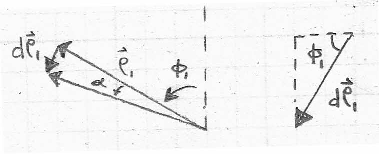
\includegraphics[width=0.6\textwidth]{Figures/Q5_P1_Rho1.pdf}}
 \subfigure[]{
 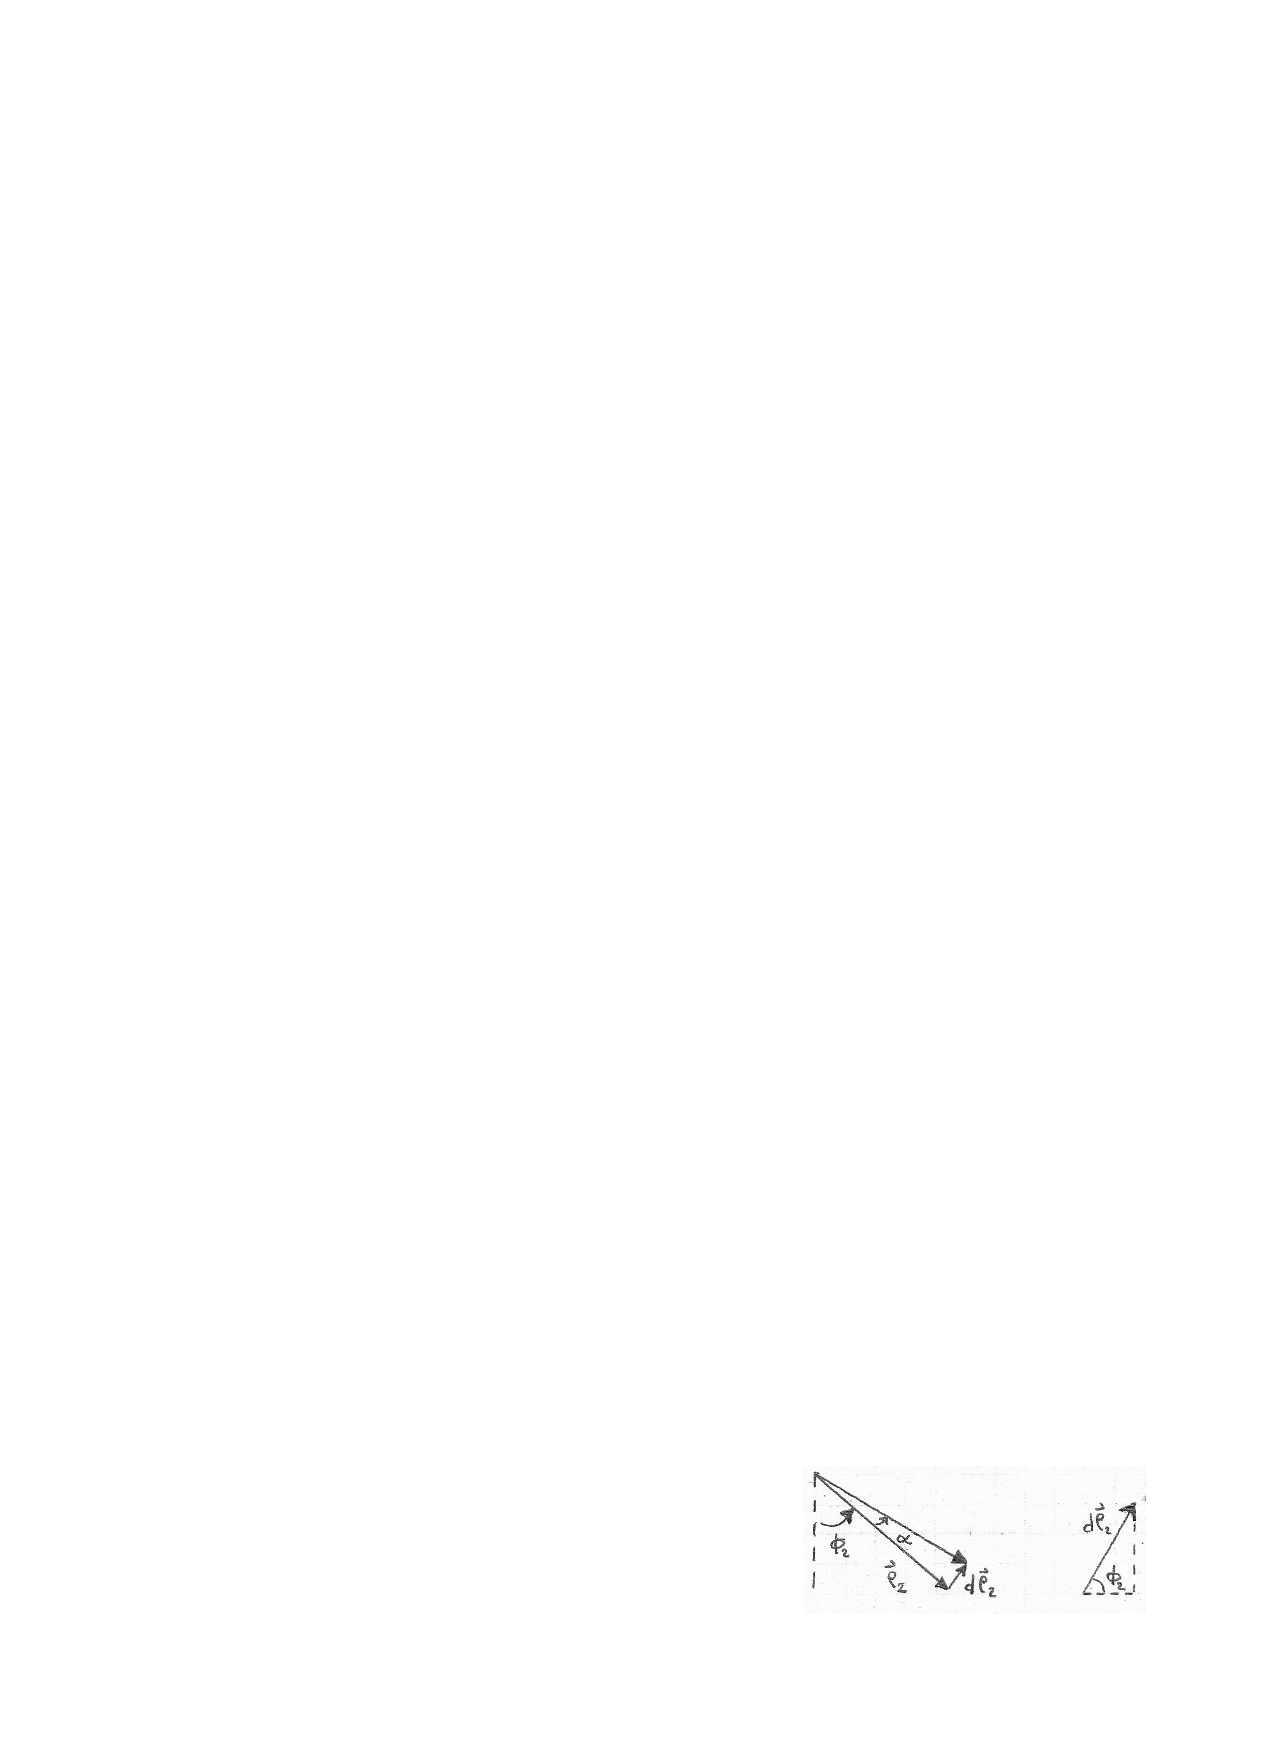
\includegraphics[width=0.5\textwidth]{Figures/Q5_P1_Rho2.pdf}}
 \caption{Rho Vectors}
 \label{drho12}
\end{figure}

\subsection*{Centroid Location}

Working with an off-axis parabolic mirror segment requires intermediate calculations to find the location of the centroid with respect to the vertex. The simulation presented assumes the $x$-coordinate of both mirror endpoints is known. First, calculate the arc length, $L$, of the mirror as follows.

\begin{equation}
\label{eq:arclength}
\centering
\begin{aligned}
	(dL)^2 &= (dx)^2 + (dy)^2 \\
	\frac{dL}{dx} &= \sqrt{1+\left(\frac{dy}{dx}\right)^2} \\
	L &= \bigintss_a^b \sqrt{1+\left(\frac{dy}{dx}\right)^2}dx
\end{aligned}
\end{equation}\

Then, find the mass of the mirror using a constant length density, $\rho_L$, and the arc length, $L$, between the known endpoint locations, $x_1$ and $x_2$.

\begin{equation}
\label{eq:mass}
\centering
\begin{aligned}
	m &= \rho_L L \\
	&= \rho_L \bigintss_{x_1}^{x_2} \sqrt{1+\left(\frac{dy}{dx}\right)^2}dx
\end{aligned}
\end{equation}\

Next, calculate the moments about the $x$- and $y$-axes. The moment is the mass of a differential element multiplied by the perpendicular distance from the axis.

\begin{equation}
\label{eq:moment1}
\centering
\begin{aligned}
	M_x &= \rho_L \bigintss_{x_1}^{x_2} y(x)\sqrt{1+\left(\frac{dy}{dx}\right)^2}dx \\
	M_y &= \rho_L \bigintss_{x_1}^{x_2} x\sqrt{1+\left(\frac{dy}{dx}\right)^2}dx
\end{aligned}
\end{equation}\

To calculate the centroid location, note that the moment about an axis is equal to the mass located at the centroid.\\

\begin{equation}
\label{eq:moment2}
\centering
\begin{aligned}
	M_x &= m\bar{y} \\
	M_y &= m\bar{x}
\end{aligned}
\end{equation}\

Thus,

\begin{equation}
\label{eq:centroid}
\centering
\begin{aligned}
	\bar{x} &= \frac{M_y}{m} \\
	&= \frac{\rho_L}{m} \bigintss_{x_1}^{x_2} x\sqrt{1+\left(\frac{dy}{dx}\right)^2}dx \\
	\\
	\bar{y} &= \frac{M_x}{m} \\
	&= \frac{\rho_L}{m} \bigintss_{x_1}^{x_2} y(x)\sqrt{1+\left(\frac{dy}{dx}\right)^2}dx
\end{aligned}
\end{equation}\

For a parabola,

\begin{equation}
\label{parabola}
\centering
\begin{aligned}
	y(x) &= \frac{1}{4f}x^2 \\
	\\
	\frac{dy}{dx} &= \frac{1}{2f}x
\end{aligned}
\end{equation}\\

$\vec{\rho}_V$, $\vec{\rho}_1$, and $\vec{\rho}_2$ of Figure~\ref{drho12} are easily calculated as the difference between the associated point position vectors.

\subsection*{Equations of Motion}

Substitute Equations~\eqref{eq:drho} into~\eqref{eq:kinemEQ}, then \eqref{eq:kinemEQ} into \eqref{eq:kinEQ} to generate equations of motion with $x$ and $y$ position of the CoM and $\alpha$ as the system states.

\begin{subequations}
\label{eq:fullEoM}
\centering
\begin{align}
	\ddot{x} &= \frac{1}{m}\left[-k\left(x - d\rho_{1_x}\right) -c\left(\dot{x} - d\dot{\rho}_{1_x}\right) - k\left(x - d\rho_{2_x}\right) -c\left(\dot{x} - d\dot{\rho}_{2_x}\right) + D_x \right]\\
	\nonumber \\
	\ddot{y} &= \frac{1}{m}\left[-k\left(y - d\rho_{1_y}\right) -c\left(\dot{y} - d\dot{\rho}_{1_y}\right) - k\left(y - d\rho_{2_y}\right) -c\left(\dot{y} - d\dot{\rho}_{2_y}\right) + D_y \right] \\
	\nonumber \\
	\begin{split}
	\ddot{\alpha} &= \frac{1}{I} \Biggl\{ \rho_{2_y}\left[-k\left(x - d\rho_{2_x}\right) - c\left(\dot{x} - d\dot{\rho}_{2_x}\right)+D_x\right] +  
													 \rho_{2_x}\left[-k\left(y - d\rho_{2_y}\right) - c\left(\dot{y} - d\dot{\rho}_{2_y}\right)+D_y\right]  \\
						&					  + \rho_{y_1}\left[-k\left(x - d\rho_{1_x}\right) - c\left(\dot{x} - d\dot{\rho}_{1_x}\right)\right] + 
													 \rho_{x_1}\left[-k\left(y - d\rho_{1_y}\right)  - c\left(\dot{y} - d\dot{\rho}_{1_y}\right)\right]  \Biggr\}
	\end{split}
\end{align}
\end{subequations}
